  \section{Experiments}
\label{sec:experiments}

In this section, we describe our HBM implementation and Ramulator simulations on several PARSEC benchmarks. We run the PARSEC v2.1 and v3.0 benchmarks suites with the gem5 simulator to generate memory traces for multicore shared memory scenarios. Next, we evaluate the performance of reorder buffer by running the memory traces through the Ramulator DRAM simulator. We extended the Ramulator simulator to include the reorder buffer. To evaluate the performance of the reorder buffer, we compare the number of CPU cycles needed for extended Ramulator to execute the CPU traces for against the unextended Ramulator simulator.

\subsection{HBM Implementation}
%\Ethan{Move all implementation details here, is sub-channel the same as pseudo channel? OK or still repetitive?}
%\Ankit{Suddenly, there is too much jargon about HBM...Have we defined all these things in the background section?}
Our coding scheme is based on a single $16$-bank channel of HBM DRAM operating in Pseudo Channel Mode ($8$ banks per pseudo channel). To fit the layout of Figure~\ref{fig:memsys} and Section~\ref{sec:codingArchitecture}, Pseudo Channel 0 is used for data banks and Pseudo Channel 1 is used for parity banks. 
%
%The pseudo channel conceptually divides the memory of a single channel in half. 
%Since this mode divides a channel into two individual $8$ bank sub-channels, we assign one sub-channel for data banks and the other sub-channel for parity banks. 
%
Wherever possible, we try to interleave the banks. This ensures that most large, linear accesses will be spread across multiple banks with reduced contention.

In this mode, the 128-bit data bus is split into 2 individual 64-bit segments. 
However, the pseudo channels share the same address and command bus: commands and addresses may be sent to one pseudo channel or the other, but not to both. They also decode and execute commands individually. For commands that are common to both pseudo channels, strict timing conditions must be met to avoid conflicts.
%The burst length is set to $4$. This means that on each segment, a read or write transaction transfers $256$ bits in a burst of four $64$-bit cycles. 
Table~\ref{tab:design_params} describes additional design details.
%
\begin{table}[h!]
 \small
  \centering
  \begin{tabular}{|c|p{5cm}|}
    \hline
    Memory overhead & Storage of parity is limited to 50\% of the overall memory. \\
    \hline
    Memory Banks & 8 Data banks, 8 parity banks \\
    \hline           
    Cache Line Size & 128/256 bytes size \\ \hline  
    Element Size & Each element is 256 bytes \\ \hline  
    Number of Cores & 6-8 cores for Wireless SoC platform \\ \hline  
    Access Rate & 1GHz memory speed \\ \hline  
    Burst Length & 4 (256-bit transfer in four 64-bit bursts)\\ \hline
  \end{tabular}
  \caption{Summary table of design parameters.}
  \label{tab:design_params}
\end{table}


\begin{remark} %[{\bf Address mapping}]
\label{rem:address}
%\Ankit{I don't see any reason to present address mapping here...or probably this needs to presented in a better manner to create coherent story.} 
Figure~\ref{fig:mapping} describes the address mapping for each channel. The least significant ``OFFSET'' bits of the address signify the byte level addressing of the data. The $6$ most significant ``CA'' bits indicate column address, the next $14$ ``RA'' bits indicate row address, the $3$ ``BA'' bits decide the bank, and the remaining $3$ ``CH'' bits specify the channel. 
\end{remark}
%%%%%%%%%%%%%%%%%%%%%%%%%%%%%%%%%%%%%%%%%%%
\begin{figure}[h!] \centering
%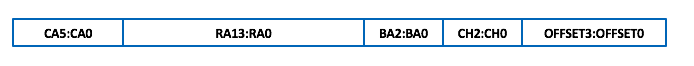
\includegraphics[width=0.95\linewidth]{figures/mapping.png} 
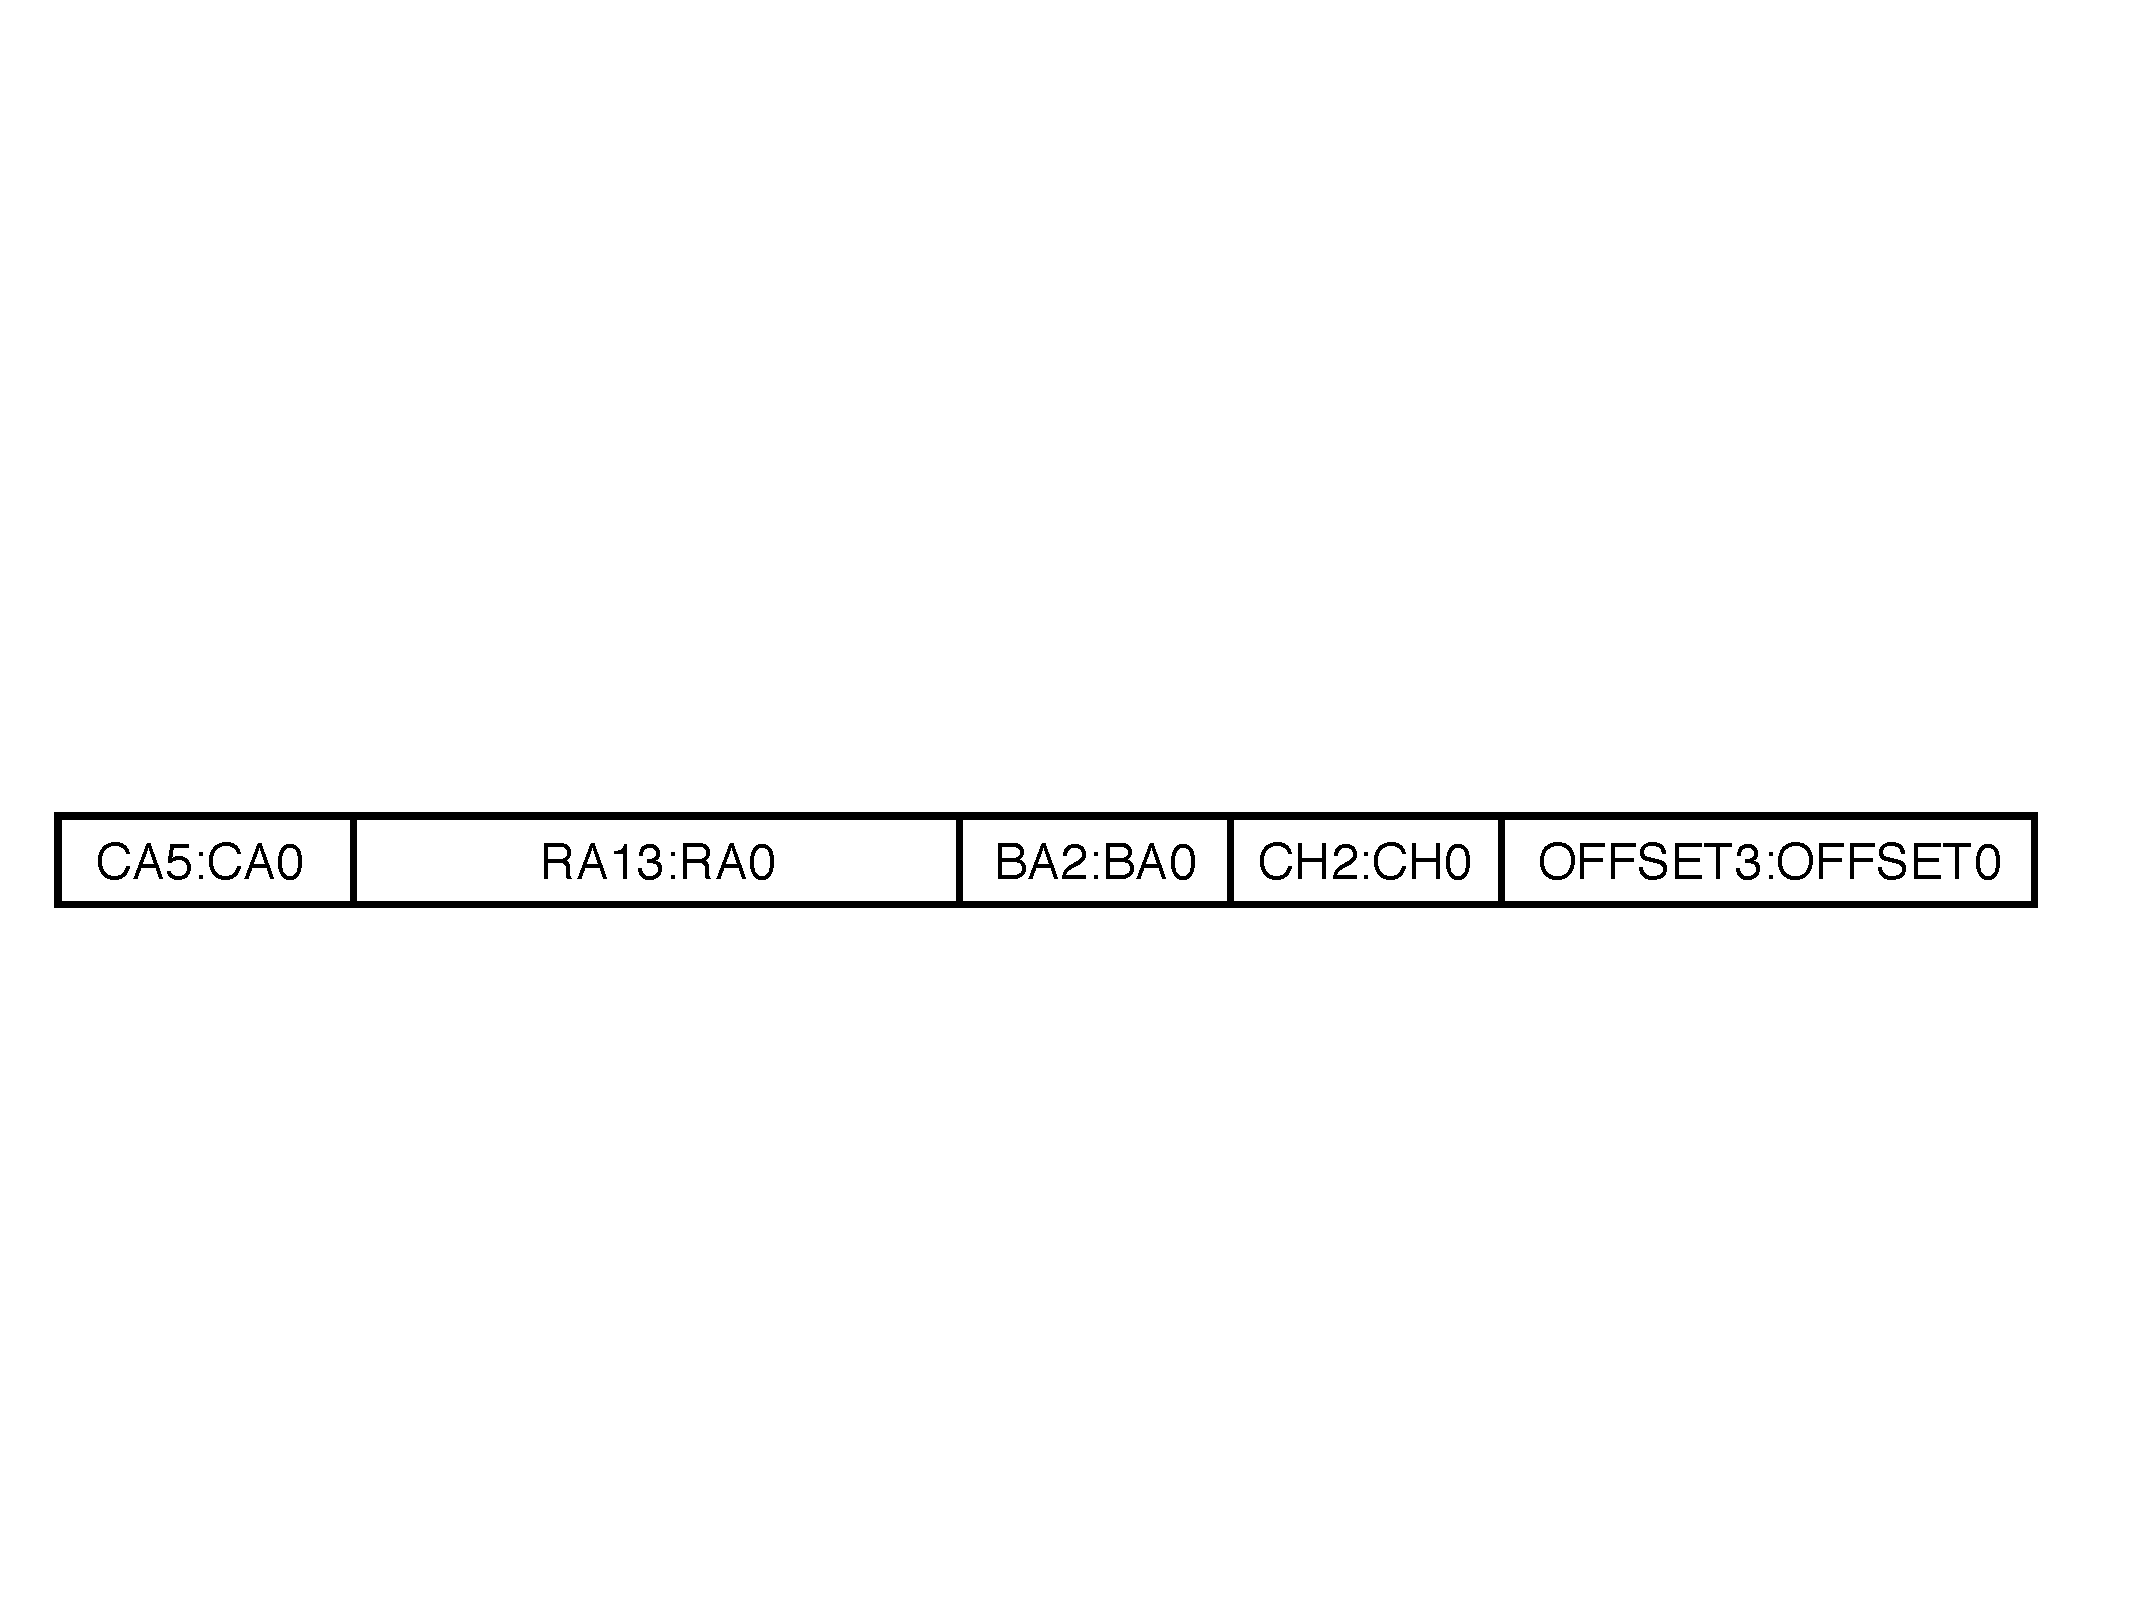
\includegraphics[width=0.98\linewidth]{figures/ChAddressing.pdf} 
\caption{Address mapping for channels.}
\label{fig:mapping}
\end{figure}
%%%%%%%%%%%%%%%%%%%%%%%%%%%%%%%%%%%%%%%%%%%


\begin{figure}[h!] \centering
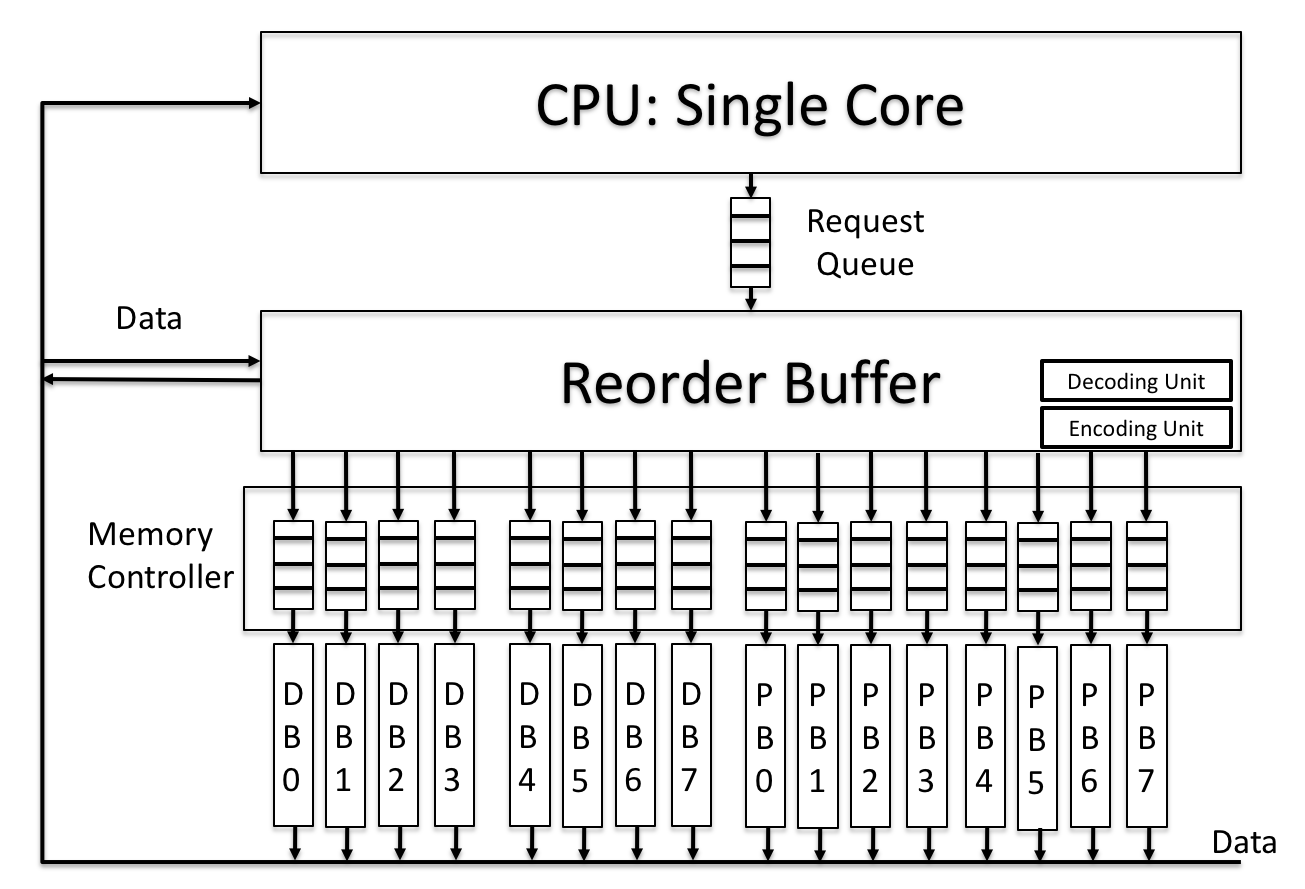
\includegraphics[width=0.9\linewidth]{figures/single-core-cpu.png} 
\caption{Single-core CPU Simulation.}
\label{fig:single-core-cpu}
\end{figure}

\begin{figure}[h!] \centering
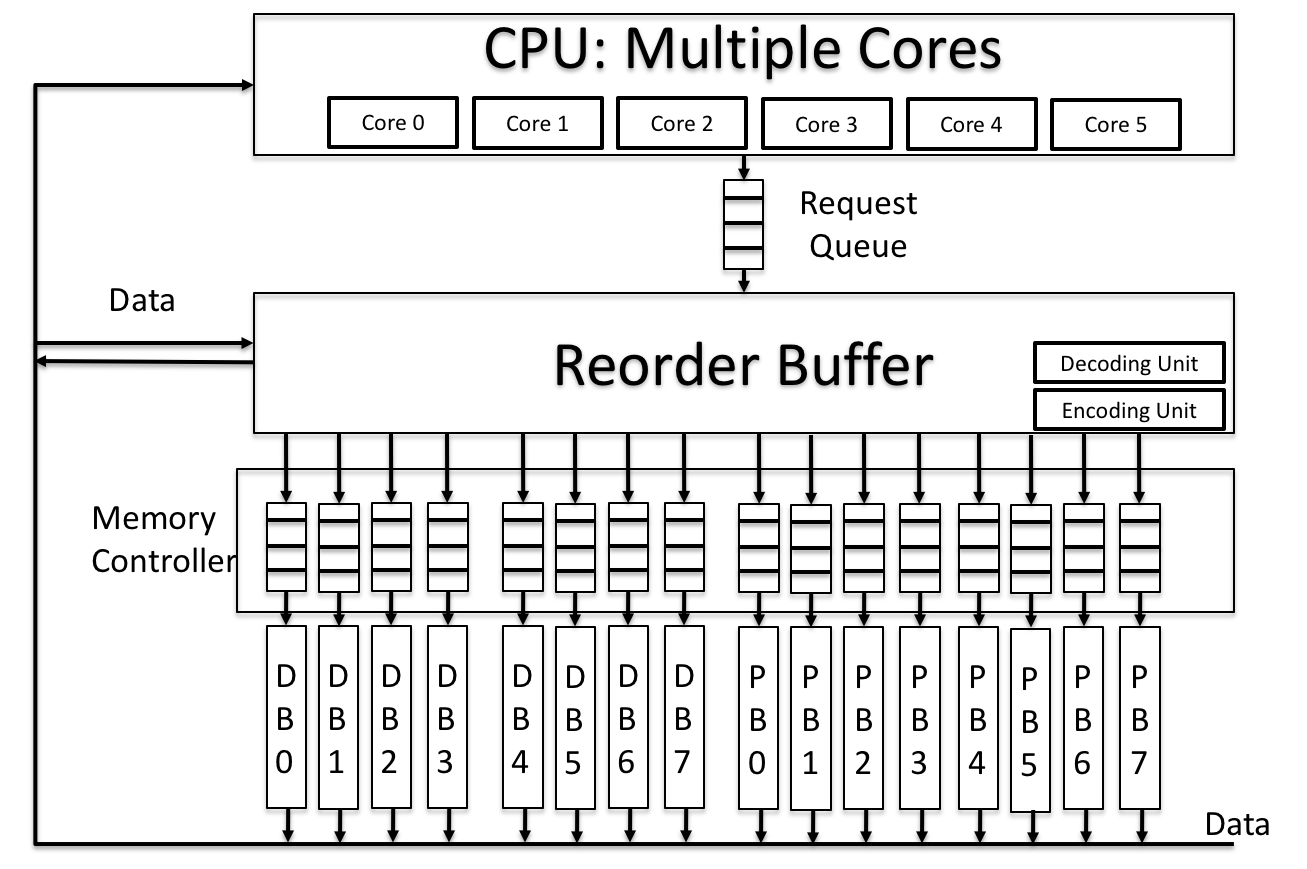
\includegraphics[width=0.9\linewidth]{figures/multi-core-cpu.png} 
\caption{Multi-core CPU Simulation.}
\label{fig:multi-core-cpu}
\end{figure}

\subsection{Memory Trace Generation}
We use the PARSEC benchmark suite to evaluate how the reorder buffer can improve performance in shared memory scenarios. The PARSEC benchmark suite was developed for Chip Multiprocessors and is composed of a diverse set of multithreaded applications. [see paper 1 for citation - this exact quote is in there as well.] We run the PARSEC benchmarks on the gem5 simulator to generate memory traces for use in evaluating the efficacy of the proposed coded model.

The gem5 simulator allows us to select a quantity of processors on which we run the PARSEC benchmarks. For most traces, we used 8 processors. We also use 16 and 32 processors to evaluate the coded model's performance on denser memory traces. The execution of the PARSEC benchmarks has a number of stages. We are only interested in the multi core shared memory stages, so we extracted this portion of trace out from the full memory trace.

We convert the gem5 memory traces to the Ramulator CPU-trace format. The conversion process merely involves removing extra information from the gem5 memory traces. The Ramulator CPU-trace requires only the read and writeback addresses for memory accesses, as well as the number of CPU cycles between the accesses.

\subsection{PARSEC Trace Attributes}
The memory traces we use to evaluate the proposed coded model must be dense because the proposed coded model is most helpful when remedying bank conflicts. The memory traces generated by gem5 with the PARSEC benchmarks are sufficiently dense, as illustrated by Figure~\ref{fig:dedup_dense}. There is an average of 1.11 nanoseconds between memory access per core. This equates to an average of 2.22 cycles between memory access requests per 2Ghz Processor.

The region of memory utilized by the picture benchmark does not change with time. Figure~\ref{fig:dedup_whole} shows an entire memory trace used to evaluate the performance of the coded model. We observe that there are two major memory bands. Figure~\ref{fig:dedup_dense} is a magnified view of the bottom band. This figure reveals that the bottom band is composed of two sub-bands of similar density. These two sub-bands contain over 90\% of the memory accesses in this memory trace. Figure~\ref{fig:dedup_dense} also shows that the memory regions used by the processors overlap to a degree which yields frequent bank conflicts.

\begin{figure}[h!]

		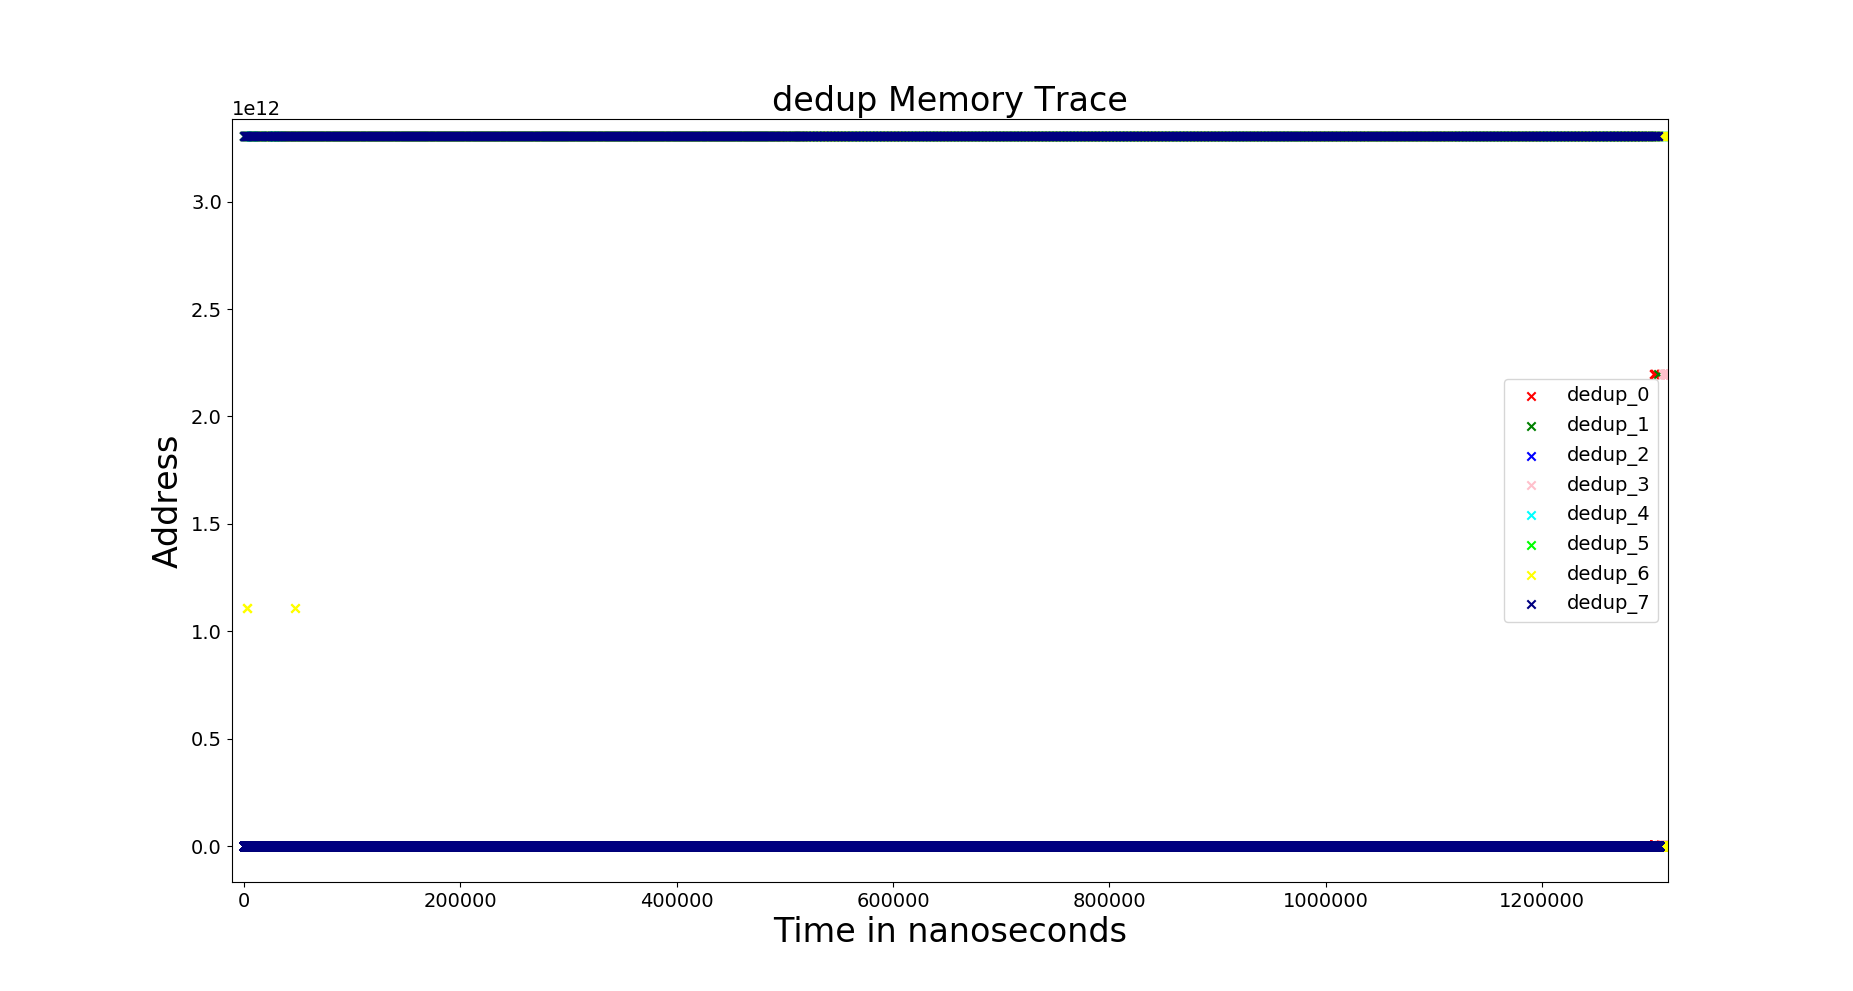
\includegraphics[width=\linewidth]{figures/dedup_whole.png}
		\caption{Memory Access from the Dedup PARSEC benchmark. This trace was generated using 8 cores.}
		\label{fig:dedup_whole}
\end{figure}

\begin{figure}[h!]
		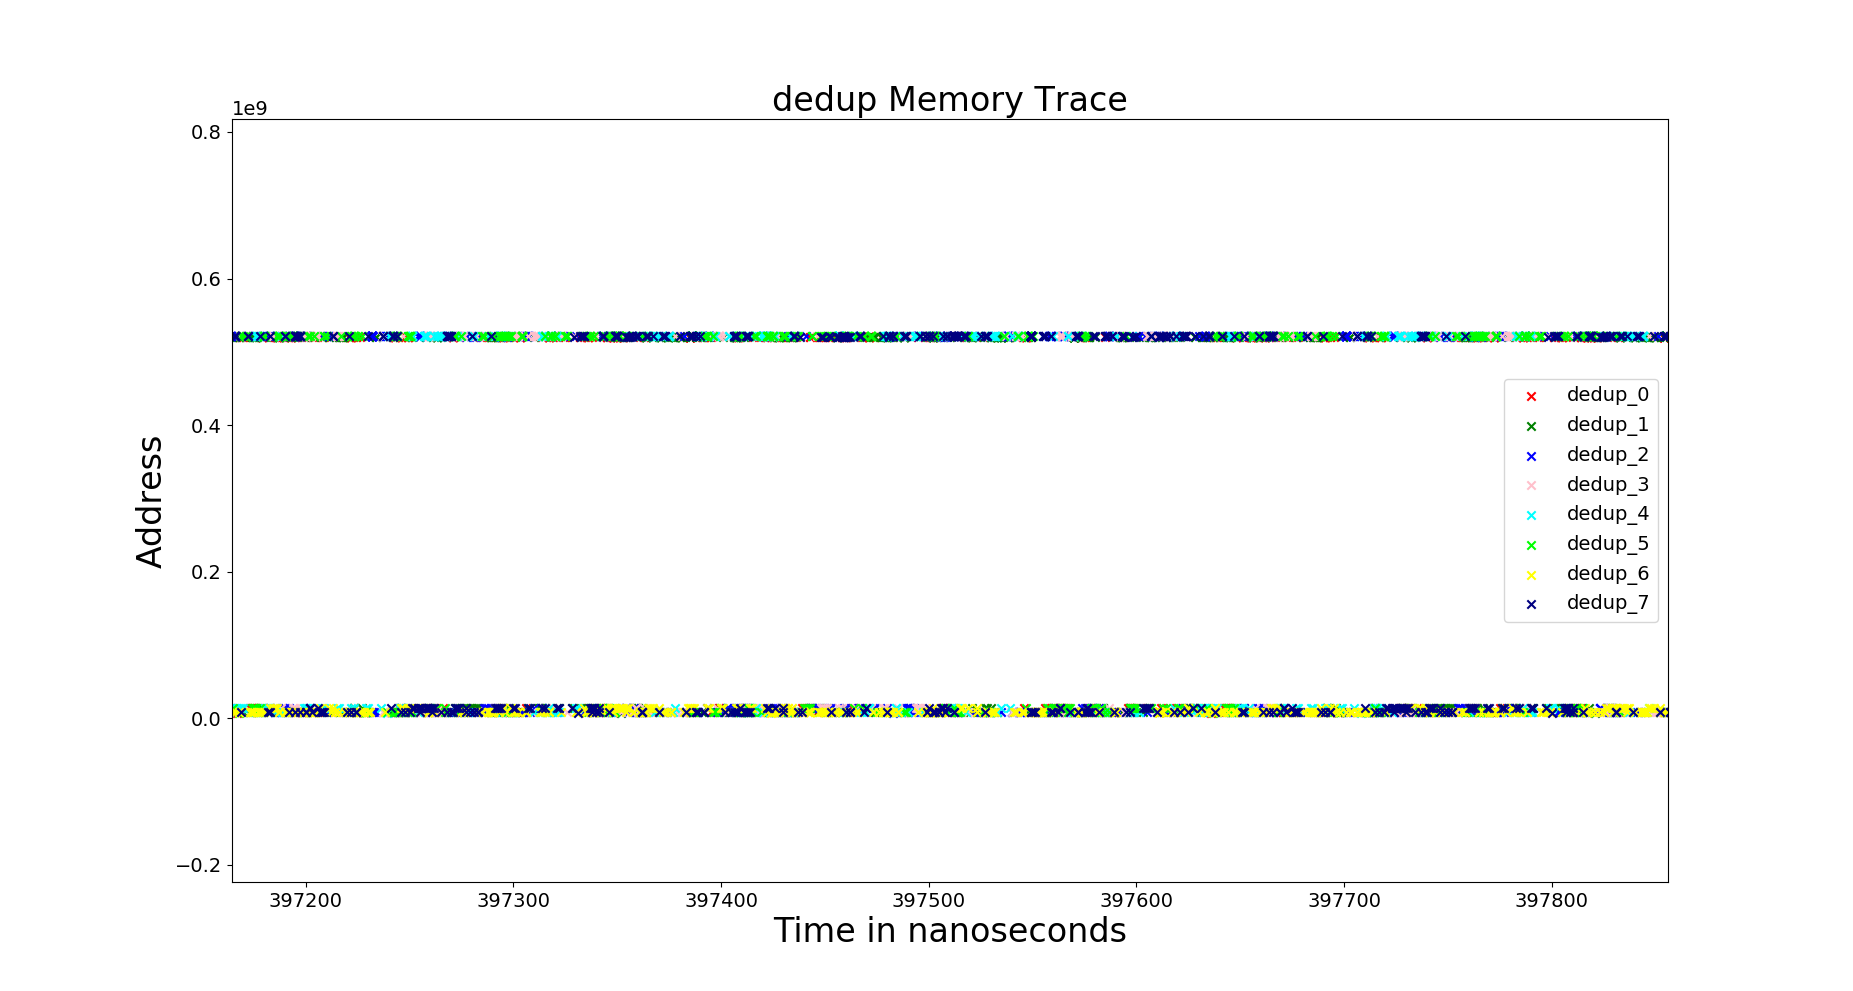
\includegraphics[width=\linewidth]{figures/dedup_dense.png}
		\caption{Memory Access from the Dedup PARSEC benchmark demonstrating the density of memory accesses}
		\label{fig:dedup_dense}
\end{figure}
		

\subsection{Ramulator}
The Ramulator DRAM simulator estimates the number of CPU cycles required by memory systems to execute a memory trace\cite{Ramulator}. We use a slightly modified version of the vanilla Ramulator to simulate the coded model without the reorder buffer or parity banks. Next, we run the simulation with the reorder buffer and parity banks implemented and we compare the results. We use a consistent Ramulator configuration across the simulations, so any differences in simulator performance is a result of the proposed coded model. We test different parity bank architectures and reorder buffer lengths. The Ramulator configuration file used to acquire the simulation results: 

\begin{itemize}
\item Standard : HBM
\item Channels: 8
\item Ranks: 1
\item Speed: 1 Gigabits per second
\item Organization: 4 Gigabits
\item CPU ticks: 32
\item Memory ticks: 5
\end{itemize}



%\Ethan{change to relative improvement like the others?} The number of cycles used for read and write accesses is shown in Figure \ref{fig:spec-cycles1} for the baseline and our coded HBM scheme assuming a reorder buffer of infinite size. This simulation further bounds the performance improvements we expect in practice because no rows are evicted from reorder buffer. For heavy access implementations like MCF, a large improvement can be seen in the reduction of cycles used to serve the requests. \Ethan{add soemthing about omnetpp, soplex, and/or sjeng}
% The subsequent Figures show the performance levels with various reorder buffer size. \par

%
%\begin{figure}[htb] \centering
%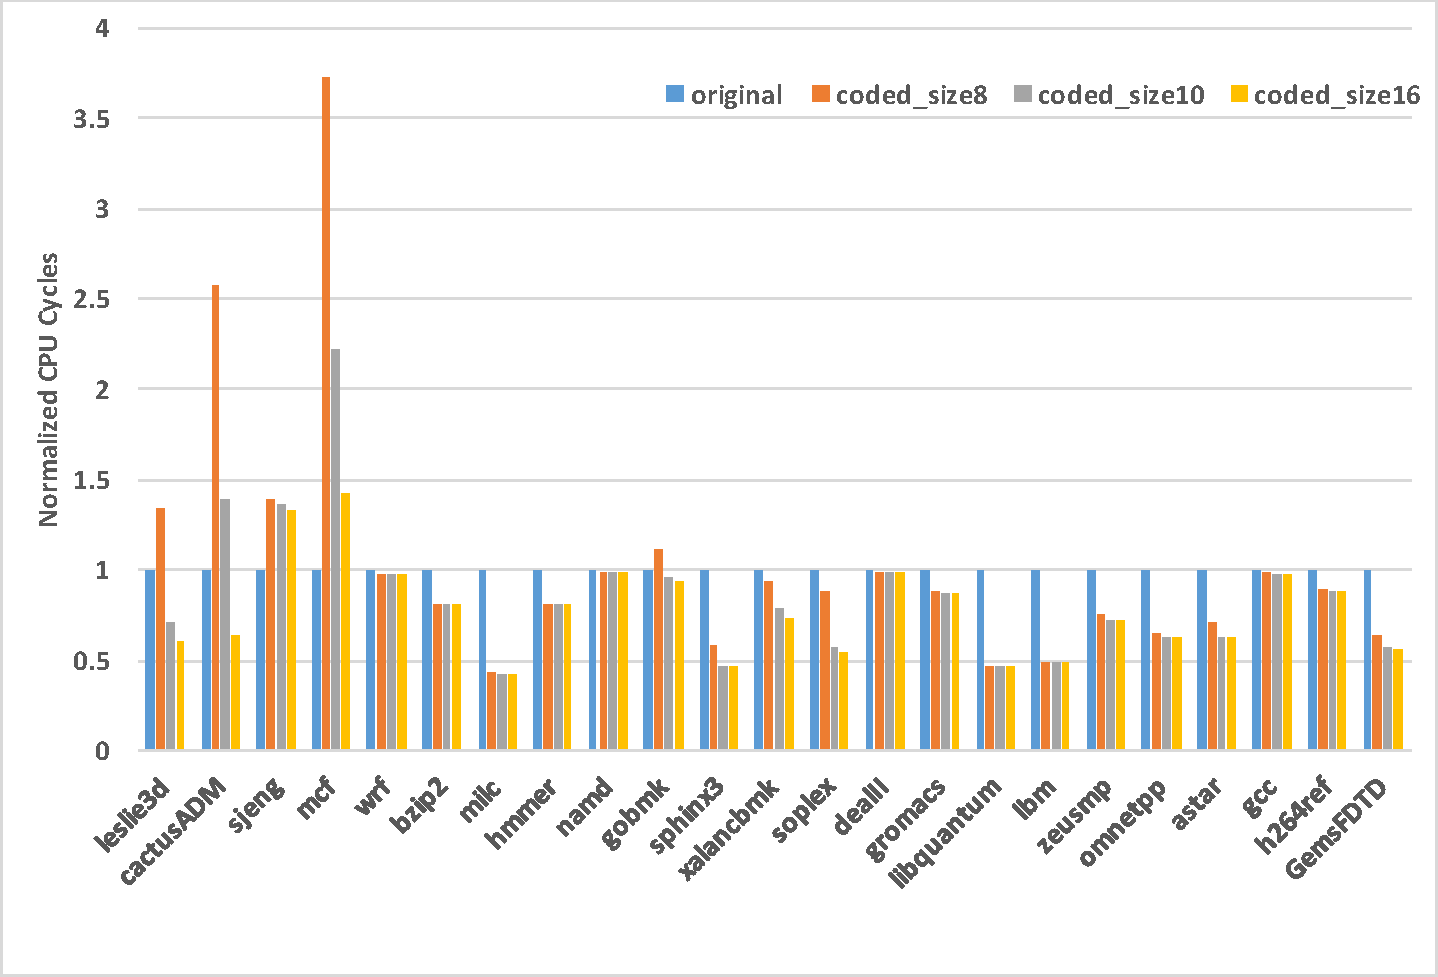
\includegraphics[width=\linewidth]{figures/spec-cycles2.pdf} 
%\caption{Simulated Number of CPU cycles: Baseline HBM versus Coded HBM across different benchmarks (with reorder buffer size of $8, 10, 16$). \Ethan{10 bits or 16 bits? label axes}}
%\label{fig:spec-cycles2}
%\end{figure}
%
%\begin{figure}[htb] \centering
%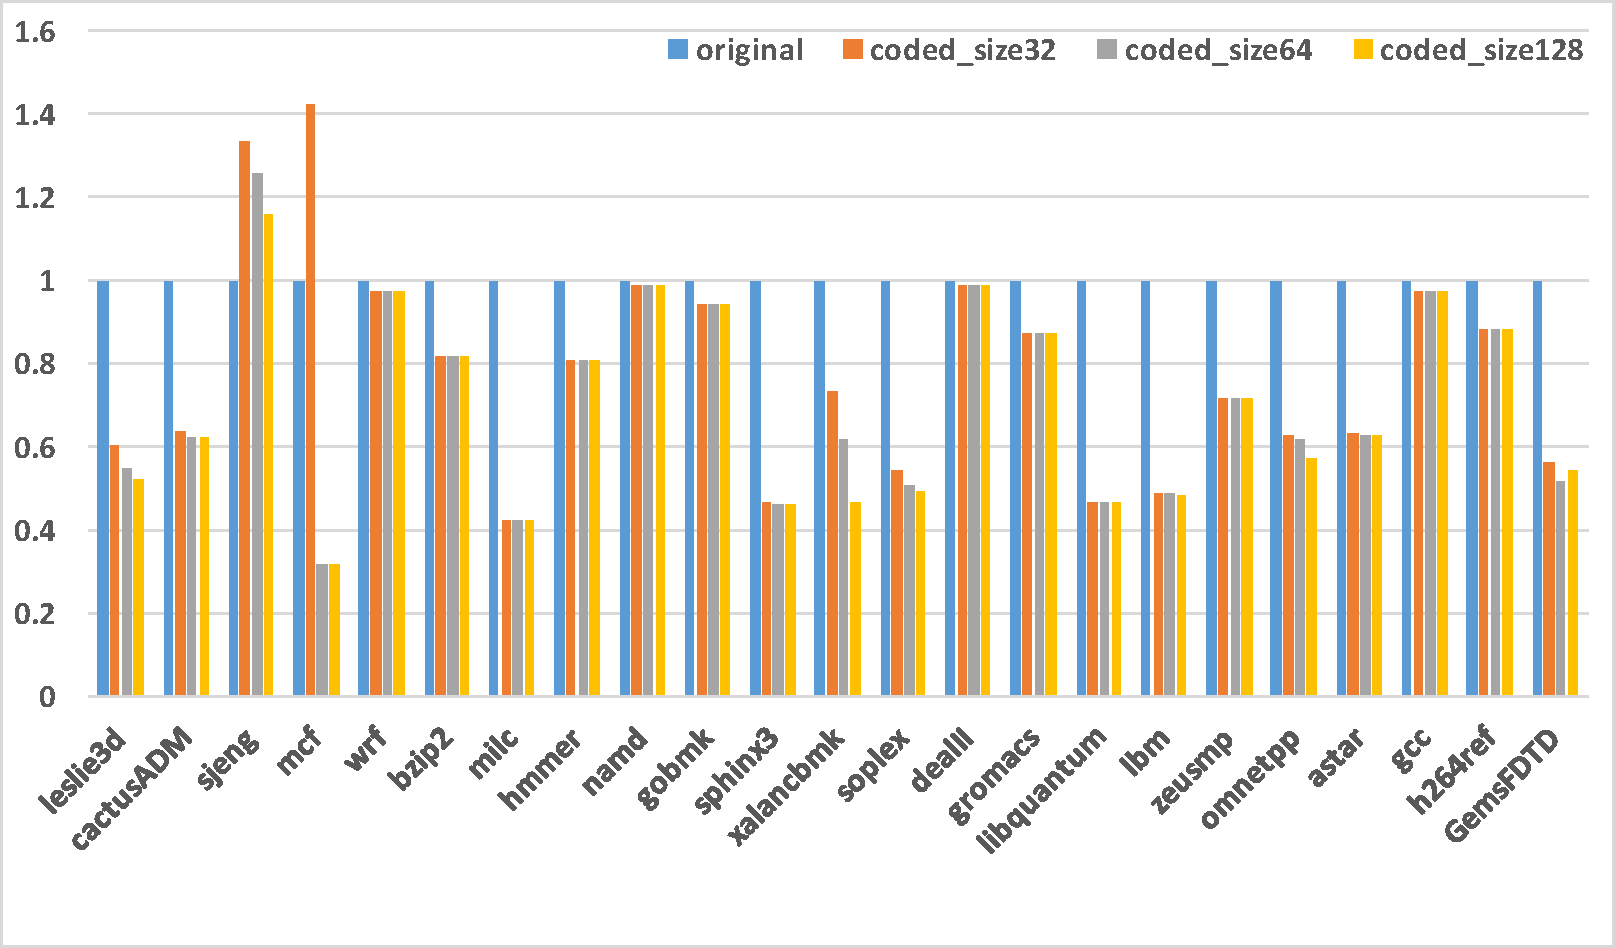
\includegraphics[width=1\linewidth]{figures/spec-cycles3.pdf} 
%\caption{Simulated Number of CPU cycles: Baseline HBM versus Coded HBM across different benchmarks (with reorder buffer size of $32, 64, 128$). \Ethan{label axes}}
%\label{fig:spec-cycles3}
%\end{figure}
%
%\begin{figure}[htb] \centering
%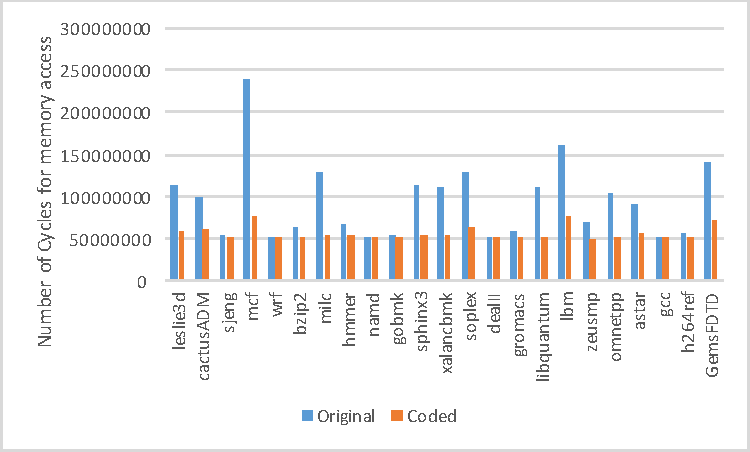
\includegraphics[width=1\linewidth]{figures/spec-cycles1.pdf} 
%\caption{Simulated Number of CPU cycles: Baseline HBM versus Coded HBM across different benchmarks (with infinite reorder buffer size). \Ethan{label axes}}
%\label{fig:spec-cycles1}
%\end{figure}

%
%\begin{figure}[htb] \centering
%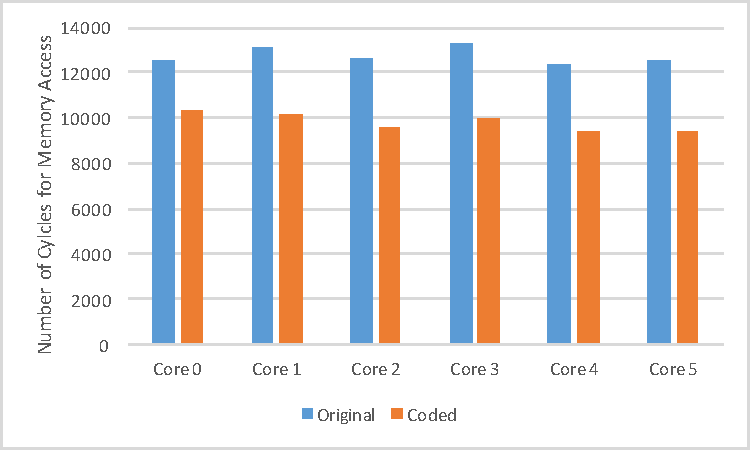
\includegraphics[width=1\linewidth]{figures/lte.pdf} 
%\caption{Simulated Number of active DRAM cycles: Baseline HBM versus Coded HBM across application-driven LTE traces (with reorder buffer size of $16$) }
%\label{fig:lte}
%\end{figure}
%
%\begin{figure}[htb] \centering
%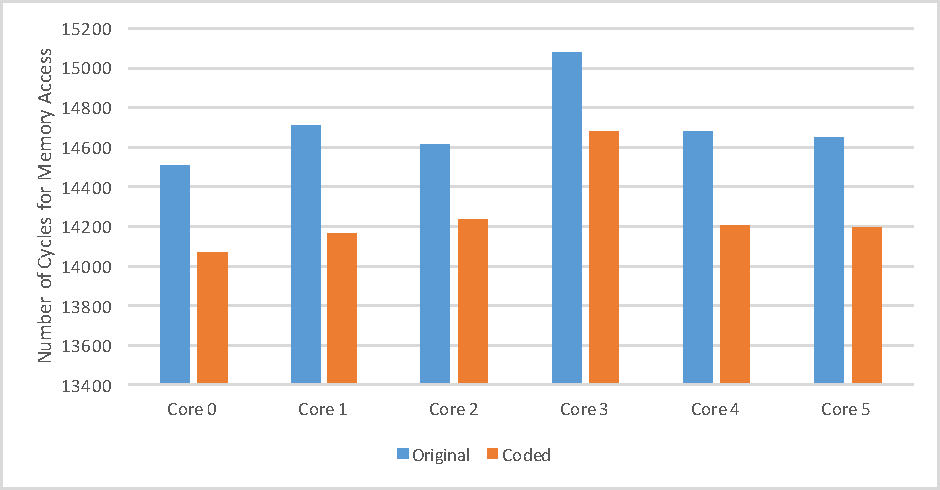
\includegraphics[width=1\linewidth]{figures/umts.pdf} 
%\caption{Simulated Number of active DRAM cycles: Baseline HBM versus Coded HBM across application-driven UTMS traces (with reorder buffer size of $16$) \Ethan{10 bits or 16 bits?}}
%\label{fig:umts}
%\end{figure}


%\subsection{Cost Analysis} 
% Table \ref{tab:size} shows the reorder buffer size as a function of depth. 
% \Ankit{This subsection is just $1$ line?!}\Ethan{Yes, explain figures more}

%\begin{table}
%\begin{tabular}{|l|l|l|l|l|l|}
%\hline \bf Depth & 8 & 16 & 32 & 64 & 128 \\ \hline
%\bf Size & 8KB & 16KB & 32.2KB & 64.5KB & 129KB \\ 
%\hline
%\end{tabular}
%\caption{Reorder Buffer Size under Different Depth}\label{tab:size}
%\end{table}

%{\color{blue} \noindent \textbf{Potential improvement using prefetching:}~
%\Ethan{Remove entire subsection?}
%We explore the implementation of a memory prefetching unit, similar to an instruction or cache prefetching unit. This unit can detect linear access patterns to regions in memory.  For example, if a string of memory accesses are issued in sequential byte sized order, then the prefetching unit will predict the next access to be in byte increments. The memory prefetching works by fetching a predicted address from the parity bank during accesses that the parity bank is idle. When future memory accesses are issued, they are first checked with the prefetched data to see if they can be used to decode any subsequent accesses memory accesses. If so, the memory access is obtained from the current accesses and prefetched data. 
%
%For example, say the prefetcher sees 2 consecutive memory requests in a row. It then predicts that the next two accesses, locations $a_0$ and $b_0$, are likely to be accessed in the near future. It reads $a_0 + b_0$ from the parity bank for future use. Next, access to location $a_0$ and $b_0$ are issued to the memory. Now, instead of reading both $a_0$ and $b_0$, only a single location has to be read from in memory, while the other location can be obtained from the prefetched data. This allows for an additional access to be issued from the now free memory bank.  In these cases, it is possible to obtain up to two additional memory accesses in a given cycle, one from the prefetched data and one from the parity bank.
%
%%Implementation of a memory prefetch should only require overhead for space and the associated logic to implement it. Since memory accesses are often stalled due to bank conflicts, checking pending accesses to the prefetched data should require no additional time overhead. As memory accesses wait to be issued in the bank queues, they can simultaneously be checked with the prefetched data. Thus, no extra latency is anticipated by the addition of a memory prefetching unit.
%
%Figure~\ref{fig:prefetch1} shows two plots of memory accesses to a bank with respect to time. The left figure shows the accesses to the memory bank by various cores. The right side figure shows a zoomed view of the accesses in the dense access region. This figure suggests the linearity of accesses. The system can look ahead in the queue to detect the consecutive address request for a memory bank and schedule a prefetch of the associated code.
%
%\noindent {\bf Coding and prefetching:~}One of the ideas explored in this paper is that of proactive prefetching of data from (unused) memory banks to buffers based on the pattern of pending access requests at the memory controller. This creates the opportunities to serve multiple access requests in a given memory cycles and also tries to utilize all the available memory banks throughout the operation of the memory system. Such prefetching based memory designs in the context of {\em uncoded} memory systems has been previously studied in the literature (see e.g.,~\cite{Kim2016, Kadjo2014, Shevgoor2015, JL2013}). To the best of our knowledge, the application of prefetching schemes with coded memory systems has not been explored before.}
